\documentclass[1p]{elsarticle_modified}
%\bibliographystyle{elsarticle-num}

%\usepackage[colorlinks]{hyperref}
%\usepackage{abbrmath_seonhwa} %\Abb, \Ascr, \Acal ,\Abf, \Afrak
\usepackage{amsfonts}
\usepackage{amssymb}
\usepackage{amsmath}
\usepackage{amsthm}
\usepackage{scalefnt}
\usepackage{amsbsy}
\usepackage{kotex}
\usepackage{caption}
\usepackage{subfig}
\usepackage{color}
\usepackage{graphicx}
\usepackage{xcolor} %% white, black, red, green, blue, cyan, magenta, yellow
\usepackage{float}
\usepackage{setspace}
\usepackage{hyperref}

\usepackage{tikz}
\usetikzlibrary{arrows}

\usepackage{multirow}
\usepackage{array} % fixed length table
\usepackage{hhline}

%%%%%%%%%%%%%%%%%%%%%
\makeatletter
\renewcommand*\env@matrix[1][\arraystretch]{%
	\edef\arraystretch{#1}%
	\hskip -\arraycolsep
	\let\@ifnextchar\new@ifnextchar
	\array{*\c@MaxMatrixCols c}}
\makeatother %https://tex.stackexchange.com/questions/14071/how-can-i-increase-the-line-spacing-in-a-matrix
%%%%%%%%%%%%%%%

\usepackage[normalem]{ulem}

\newcommand{\msout}[1]{\ifmmode\text{\sout{\ensuremath{#1}}}\else\sout{#1}\fi}
%SOURCE: \msout is \stkout macro in https://tex.stackexchange.com/questions/20609/strikeout-in-math-mode

\newcommand{\cancel}[1]{
	\ifmmode
	{\color{red}\msout{#1}}
	\else
	{\color{red}\sout{#1}}
	\fi
}

\newcommand{\add}[1]{
	{\color{blue}\uwave{#1}}
}

\newcommand{\replace}[2]{
	\ifmmode
	{\color{red}\msout{#1}}{\color{blue}\uwave{#2}}
	\else
	{\color{red}\sout{#1}}{\color{blue}\uwave{#2}}
	\fi
}

\newcommand{\Sol}{\mathcal{S}} %segment
\newcommand{\D}{D} %diagram
\newcommand{\A}{\mathcal{A}} %arc


%%%%%%%%%%%%%%%%%%%%%%%%%%%%%5 test

\def\sl{\operatorname{\textup{SL}}(2,\Cbb)}
\def\psl{\operatorname{\textup{PSL}}(2,\Cbb)}
\def\quan{\mkern 1mu \triangleright \mkern 1mu}

\theoremstyle{definition}
\newtheorem{thm}{Theorem}[section]
\newtheorem{prop}[thm]{Proposition}
\newtheorem{lem}[thm]{Lemma}
\newtheorem{ques}[thm]{Question}
\newtheorem{cor}[thm]{Corollary}
\newtheorem{defn}[thm]{Definition}
\newtheorem{exam}[thm]{Example}
\newtheorem{rmk}[thm]{Remark}
\newtheorem{alg}[thm]{Algorithm}

\newcommand{\I}{\sqrt{-1}}
\begin{document}

%\begin{frontmatter}
%
%\title{Boundary parabolic representations of knots up to 8 crossings}
%
%%% Group authors per affiliation:
%\author{Yunhi Cho} 
%\address{Department of Mathematics, University of Seoul, Seoul, Korea}
%\ead{yhcho@uos.ac.kr}
%
%
%\author{Seonhwa Kim} %\fnref{s_kim}}
%\address{Center for Geometry and Physics, Institute for Basic Science, Pohang, 37673, Korea}
%\ead{ryeona17@ibs.re.kr}
%
%\author{Hyuk Kim}
%\address{Department of Mathematical Sciences, Seoul National University, Seoul 08826, Korea}
%\ead{hyukkim@snu.ac.kr}
%
%\author{Seokbeom Yoon}
%\address{Department of Mathematical Sciences, Seoul National University, Seoul, 08826,  Korea}
%\ead{sbyoon15@snu.ac.kr}
%
%\begin{abstract}
%We find all boundary parabolic representation of knots up to 8 crossings.
%
%\end{abstract}
%\begin{keyword}
%    \MSC[2010] 57M25 
%\end{keyword}
%
%\end{frontmatter}

%\linenumbers
%\tableofcontents
%
\newcommand\colored[1]{\textcolor{white}{\rule[-0.35ex]{0.8em}{1.4ex}}\kern-0.8em\color{red} #1}%
%\newcommand\colored[1]{\textcolor{white}{ #1}\kern-2.17ex	\textcolor{white}{ #1}\kern-1.81ex	\textcolor{white}{ #1}\kern-2.15ex\color{red}#1	}

{\Large $\underline{12a_{1277}~(K12a_{1277})}$}

\setlength{\tabcolsep}{10pt}
\renewcommand{\arraystretch}{1.6}
\vspace{1cm}\begin{tabular}{m{100pt}>{\centering\arraybackslash}m{274pt}}
\multirow{5}{120pt}{
	\centering
	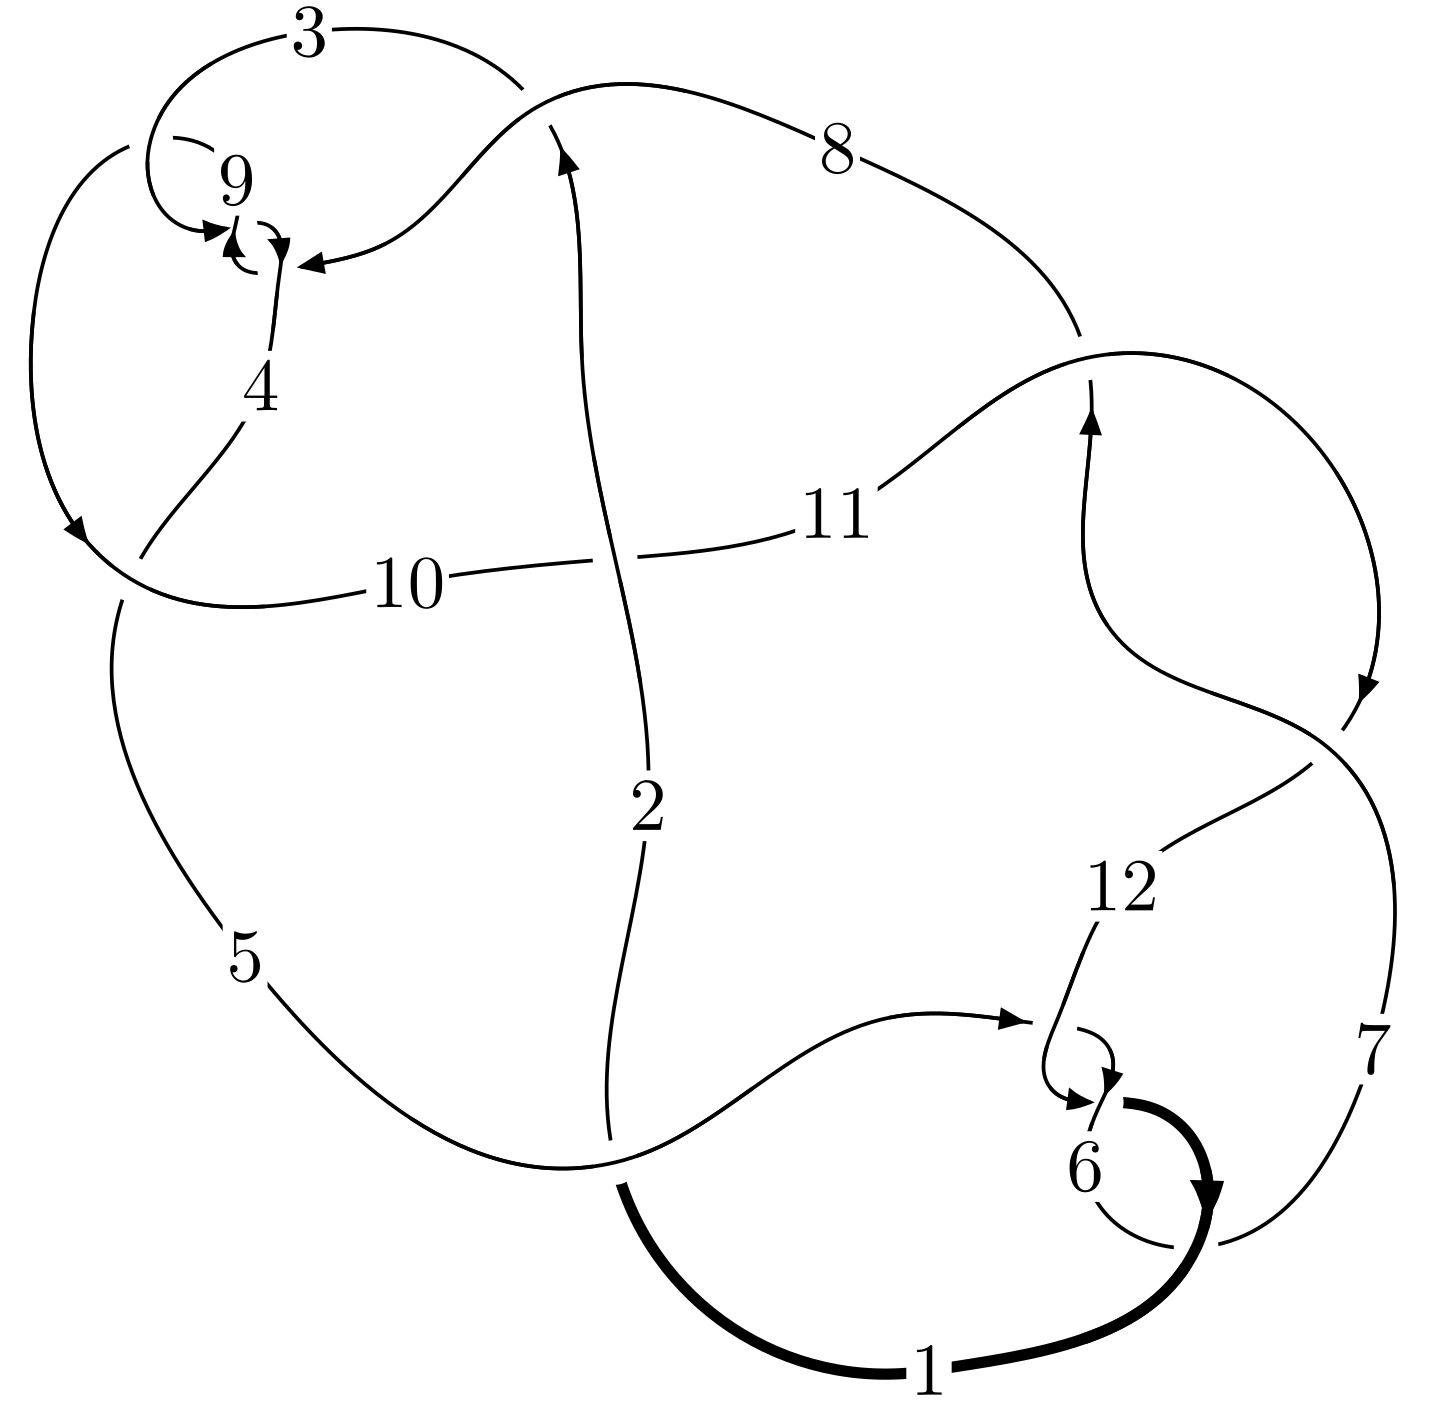
\includegraphics[width=112pt]{../../../GIT/diagram.site/Diagrams/png/2078_12a_1277.png}\\
\ \ \ A knot diagram\footnotemark}&
\allowdisplaybreaks
\textbf{Linearized knot diagam} \\
\cline{2-2}
 &
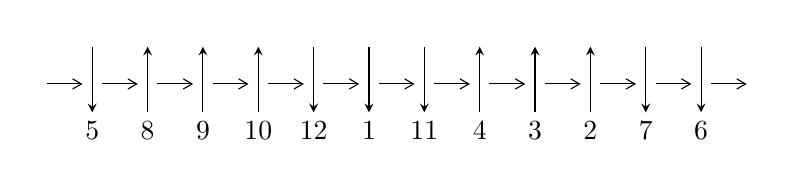
\begin{tikzpicture}[x=20pt, y=17pt]
	% nodes
	\node (C0) at (0, 0) {};
	\node (C1) at (1, 0) {};
	\node (C1U) at (1, +1) {};
	\node (C1D) at (1, -1) {5};

	\node (C2) at (2, 0) {};
	\node (C2U) at (2, +1) {};
	\node (C2D) at (2, -1) {8};

	\node (C3) at (3, 0) {};
	\node (C3U) at (3, +1) {};
	\node (C3D) at (3, -1) {9};

	\node (C4) at (4, 0) {};
	\node (C4U) at (4, +1) {};
	\node (C4D) at (4, -1) {10};

	\node (C5) at (5, 0) {};
	\node (C5U) at (5, +1) {};
	\node (C5D) at (5, -1) {12};

	\node (C6) at (6, 0) {};
	\node (C6U) at (6, +1) {};
	\node (C6D) at (6, -1) {1};

	\node (C7) at (7, 0) {};
	\node (C7U) at (7, +1) {};
	\node (C7D) at (7, -1) {11};

	\node (C8) at (8, 0) {};
	\node (C8U) at (8, +1) {};
	\node (C8D) at (8, -1) {4};

	\node (C9) at (9, 0) {};
	\node (C9U) at (9, +1) {};
	\node (C9D) at (9, -1) {3};

	\node (C10) at (10, 0) {};
	\node (C10U) at (10, +1) {};
	\node (C10D) at (10, -1) {2};

	\node (C11) at (11, 0) {};
	\node (C11U) at (11, +1) {};
	\node (C11D) at (11, -1) {7};

	\node (C12) at (12, 0) {};
	\node (C12U) at (12, +1) {};
	\node (C12D) at (12, -1) {6};
	\node (C13) at (13, 0) {};

	% arrows
	\draw[->,>={angle 60}]
	(C0) edge (C1) (C1) edge (C2) (C2) edge (C3) (C3) edge (C4) (C4) edge (C5) (C5) edge (C6) (C6) edge (C7) (C7) edge (C8) (C8) edge (C9) (C9) edge (C10) (C10) edge (C11) (C11) edge (C12) (C12) edge (C13) ;	\draw[->,>=stealth]
	(C1U) edge (C1D) (C2D) edge (C2U) (C3D) edge (C3U) (C4D) edge (C4U) (C5U) edge (C5D) (C6U) edge (C6D) (C7U) edge (C7D) (C8D) edge (C8U) (C9D) edge (C9U) (C10D) edge (C10U) (C11U) edge (C11D) (C12U) edge (C12D) ;
	\end{tikzpicture} \\
\hhline{~~} \\& 
\textbf{Solving Sequence} \\ \cline{2-2} 
 &
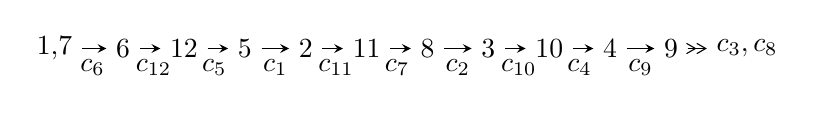
\begin{tikzpicture}[x=22pt, y=7pt]
	% node
	\node (A0) at (-1/8, 0) {1,7};
	\node (A1) at (1, 0) {6};
	\node (A2) at (2, 0) {12};
	\node (A3) at (3, 0) {5};
	\node (A4) at (4, 0) {2};
	\node (A5) at (5, 0) {11};
	\node (A6) at (6, 0) {8};
	\node (A7) at (7, 0) {3};
	\node (A8) at (8, 0) {10};
	\node (A9) at (9, 0) {4};
	\node (A10) at (10, 0) {9};
	\node (C1) at (1/2, -1) {$c_{6}$};
	\node (C2) at (3/2, -1) {$c_{12}$};
	\node (C3) at (5/2, -1) {$c_{5}$};
	\node (C4) at (7/2, -1) {$c_{1}$};
	\node (C5) at (9/2, -1) {$c_{11}$};
	\node (C6) at (11/2, -1) {$c_{7}$};
	\node (C7) at (13/2, -1) {$c_{2}$};
	\node (C8) at (15/2, -1) {$c_{10}$};
	\node (C9) at (17/2, -1) {$c_{4}$};
	\node (C10) at (19/2, -1) {$c_{9}$};
	\node (A11) at (45/4, 0) {$c_{3},c_{8}$};

	% edge
	\draw[->,>=stealth]	
	(A0) edge (A1) (A1) edge (A2) (A2) edge (A3) (A3) edge (A4) (A4) edge (A5) (A5) edge (A6) (A6) edge (A7) (A7) edge (A8) (A8) edge (A9) (A9) edge (A10) ;
	\draw[->>,>={angle 60}]	
	(A10) edge (A11);
\end{tikzpicture} \\ 

\end{tabular} \\

\footnotetext{
The image of knot diagram is generated by the software ``\textbf{Draw programme}" developed by Andrew Bartholomew(\url{http://www.layer8.co.uk/maths/draw/index.htm\#Running-draw}), where we modified some parts for our purpose(\url{https://github.com/CATsTAILs/LinksPainter}).
}\phantom \\ \newline 
\centering \textbf{Ideals for irreducible components\footnotemark of $X_{\text{par}}$} 
 
\begin{align*}
I^u_{1}&=\langle 
u^{60}+u^{59}+\cdots-2 u+1\rangle \\
\\
\end{align*}
\raggedright * 1 irreducible components of $\dim_{\mathbb{C}}=0$, with total 60 representations.\\
\footnotetext{All coefficients of polynomials are rational numbers. But the coefficients are sometimes approximated in decimal forms when there is not enough margin.}
\newpage
\renewcommand{\arraystretch}{1}
\centering \section*{I. $I^u_{1}= \langle u^{60}+u^{59}+\cdots-2 u+1 \rangle$}
\flushleft \textbf{(i) Arc colorings}\\
\begin{tabular}{m{7pt} m{180pt} m{7pt} m{180pt} }
\flushright $a_{1}=$&$\begin{pmatrix}0\\u\end{pmatrix}$ \\
\flushright $a_{7}=$&$\begin{pmatrix}1\\0\end{pmatrix}$ \\
\flushright $a_{6}=$&$\begin{pmatrix}1\\- u^2\end{pmatrix}$ \\
\flushright $a_{12}=$&$\begin{pmatrix}u\\- u^3+u\end{pmatrix}$ \\
\flushright $a_{5}=$&$\begin{pmatrix}- u^2+1\\u^4-2 u^2\end{pmatrix}$ \\
\flushright $a_{2}=$&$\begin{pmatrix}- u^5+2 u^3- u\\u^7-3 u^5+2 u^3+u\end{pmatrix}$ \\
\flushright $a_{11}=$&$\begin{pmatrix}- u^3+2 u\\- u^3+u\end{pmatrix}$ \\
\flushright $a_{8}=$&$\begin{pmatrix}u^6-3 u^4+2 u^2+1\\u^6-2 u^4+u^2\end{pmatrix}$ \\
\flushright $a_{3}=$&$\begin{pmatrix}u^{19}-8 u^{17}+26 u^{15}-40 u^{13}+19 u^{11}+24 u^9-30 u^7+9 u^3\\u^{19}-7 u^{17}+20 u^{15}-27 u^{13}+11 u^{11}+13 u^9-14 u^7+3 u^3+u\end{pmatrix}$ \\
\flushright $a_{10}=$&$\begin{pmatrix}u^{15}-6 u^{13}+14 u^{11}-14 u^9+2 u^7+6 u^5-4 u^3+2 u\\- u^{17}+7 u^{15}-19 u^{13}+22 u^{11}-3 u^9-14 u^7+6 u^5+2 u^3+u\end{pmatrix}$ \\
\flushright $a_{4}=$&$\begin{pmatrix}u^{28}-11 u^{26}+\cdots+u^2+1\\- u^{30}+12 u^{28}+\cdots+8 u^4- u^2\end{pmatrix}$ \\
\flushright $a_{9}=$&$\begin{pmatrix}u^{55}-22 u^{53}+\cdots-4 u^3+2 u\\u^{55}-21 u^{53}+\cdots+4 u^3+u\end{pmatrix}$\\&\end{tabular}
\flushleft \textbf{(ii) Obstruction class $= -1$}\\~\\
\flushleft \textbf{(iii) Cusp Shapes $= 4 u^{58}-92 u^{56}+\cdots+28 u-6$}\\~\\
\newpage\renewcommand{\arraystretch}{1}
\flushleft \textbf{(iv) u-Polynomials at the component}\newline \\
\begin{tabular}{m{50pt}|m{274pt}}
Crossings & \hspace{64pt}u-Polynomials at each crossing \\
\hline $$\begin{aligned}c_{1},c_{7},c_{11}\end{aligned}$$&$\begin{aligned}
&u^{60}+3 u^{59}+\cdots+2 u+1
\end{aligned}$\\
\hline $$\begin{aligned}c_{2},c_{4}\end{aligned}$$&$\begin{aligned}
&u^{60}- u^{59}+\cdots-30 u+53
\end{aligned}$\\
\hline $$\begin{aligned}c_{3},c_{8},c_{9}\end{aligned}$$&$\begin{aligned}
&u^{60}+u^{59}+\cdots+3 u^2+1
\end{aligned}$\\
\hline $$\begin{aligned}c_{5},c_{6},c_{12}\end{aligned}$$&$\begin{aligned}
&u^{60}- u^{59}+\cdots+2 u+1
\end{aligned}$\\
\hline $$\begin{aligned}c_{10}\end{aligned}$$&$\begin{aligned}
&u^{60}-7 u^{59}+\cdots+418 u+121
\end{aligned}$\\
\hline
\end{tabular}\\~\\
\newpage\renewcommand{\arraystretch}{1}
\flushleft \textbf{(v) Riley Polynomials at the component}\newline \\
\begin{tabular}{m{50pt}|m{274pt}}
Crossings & \hspace{64pt}Riley Polynomials at each crossing \\
\hline $$\begin{aligned}c_{1},c_{7},c_{11}\end{aligned}$$&$\begin{aligned}
&y^{60}+61 y^{59}+\cdots-34 y+1
\end{aligned}$\\
\hline $$\begin{aligned}c_{2},c_{4}\end{aligned}$$&$\begin{aligned}
&y^{60}-43 y^{59}+\cdots+30370 y+2809
\end{aligned}$\\
\hline $$\begin{aligned}c_{3},c_{8},c_{9}\end{aligned}$$&$\begin{aligned}
&y^{60}+49 y^{59}+\cdots+6 y+1
\end{aligned}$\\
\hline $$\begin{aligned}c_{5},c_{6},c_{12}\end{aligned}$$&$\begin{aligned}
&y^{60}-47 y^{59}+\cdots+6 y+1
\end{aligned}$\\
\hline $$\begin{aligned}c_{10}\end{aligned}$$&$\begin{aligned}
&y^{60}-19 y^{59}+\cdots+581526 y+14641
\end{aligned}$\\
\hline
\end{tabular}\\~\\
\newpage\flushleft \textbf{(vi) Complex Volumes and Cusp Shapes}
$$\begin{array}{c|c|c}  
\text{Solutions to }I^u_{1}& \I (\text{vol} + \sqrt{-1}CS) & \text{Cusp shape}\\
 \hline 
\begin{aligned}
u &= \phantom{-}0.952891 + 0.114591 I\end{aligned}
 & -1.63134 - 3.97089 I & \phantom{-0.000000 -}0. + 3.95693 I \\ \hline\begin{aligned}
u &= \phantom{-}0.952891 - 0.114591 I\end{aligned}
 & -1.63134 + 3.97089 I & \phantom{-0.000000 } 0. - 3.95693 I \\ \hline\begin{aligned}
u &= -0.913578\phantom{ +0.000000I}\end{aligned}
 & \phantom{-}2.26750\phantom{ +0.000000I} & \phantom{-}4.34250\phantom{ +0.000000I} \\ \hline\begin{aligned}
u &= -0.046410 + 0.879087 I\end{aligned}
 & \phantom{-}11.14760 + 5.09122 I & \phantom{-}7.88188 - 3.54555 I \\ \hline\begin{aligned}
u &= -0.046410 - 0.879087 I\end{aligned}
 & \phantom{-}11.14760 - 5.09122 I & \phantom{-}7.88188 + 3.54555 I \\ \hline\begin{aligned}
u &= \phantom{-}0.036027 + 0.879552 I\end{aligned}
 & \phantom{-}7.90629 - 0.72735 I & \phantom{-}4.83751 - 0.28515 I \\ \hline\begin{aligned}
u &= \phantom{-}0.036027 - 0.879552 I\end{aligned}
 & \phantom{-}7.90629 + 0.72735 I & \phantom{-}4.83751 + 0.28515 I \\ \hline\begin{aligned}
u &= \phantom{-}0.054075 + 0.877605 I\end{aligned}
 & \phantom{-}6.64512 - 9.38838 I & \phantom{-}3.45721 + 5.82134 I \\ \hline\begin{aligned}
u &= \phantom{-}0.054075 - 0.877605 I\end{aligned}
 & \phantom{-}6.64512 + 9.38838 I & \phantom{-}3.45721 - 5.82134 I \\ \hline\begin{aligned}
u &= \phantom{-}0.014493 + 0.848975 I\end{aligned}
 & \phantom{-}5.96433 - 1.64461 I & \phantom{-}4.63229 + 3.99521 I \\ \hline\begin{aligned}
u &= \phantom{-}0.014493 - 0.848975 I\end{aligned}
 & \phantom{-}5.96433 + 1.64461 I & \phantom{-}4.63229 - 3.99521 I \\ \hline\begin{aligned}
u &= -0.039777 + 0.829212 I\end{aligned}
 & \phantom{-}0.36934 + 3.43260 I & -0.37711 - 3.47540 I \\ \hline\begin{aligned}
u &= -0.039777 - 0.829212 I\end{aligned}
 & \phantom{-}0.36934 - 3.43260 I & -0.37711 + 3.47540 I \\ \hline\begin{aligned}
u &= \phantom{-}1.261800 + 0.016743 I\end{aligned}
 & -2.82969 - 0.00473 I & \phantom{-0.000000 } 0 \\ \hline\begin{aligned}
u &= \phantom{-}1.261800 - 0.016743 I\end{aligned}
 & -2.82969 + 0.00473 I & \phantom{-0.000000 } 0 \\ \hline\begin{aligned}
u &= -1.277440 + 0.123654 I\end{aligned}
 & -4.34670 + 2.46287 I & \phantom{-0.000000 } 0 \\ \hline\begin{aligned}
u &= -1.277440 - 0.123654 I\end{aligned}
 & -4.34670 - 2.46287 I & \phantom{-0.000000 } 0 \\ \hline\begin{aligned}
u &= -1.237020 + 0.366524 I\end{aligned}
 & -3.32294 + 0.86956 I & \phantom{-0.000000 } 0 \\ \hline\begin{aligned}
u &= -1.237020 - 0.366524 I\end{aligned}
 & -3.32294 - 0.86956 I & \phantom{-0.000000 } 0 \\ \hline\begin{aligned}
u &= -1.277970 + 0.198182 I\end{aligned}
 & -4.03371 + 1.65180 I & \phantom{-0.000000 } 0 \\ \hline\begin{aligned}
u &= -1.277970 - 0.198182 I\end{aligned}
 & -4.03371 - 1.65180 I & \phantom{-0.000000 } 0 \\ \hline\begin{aligned}
u &= \phantom{-}1.226230 + 0.424129 I\end{aligned}
 & \phantom{-}3.02962 + 4.73104 I & \phantom{-0.000000 } 0 \\ \hline\begin{aligned}
u &= \phantom{-}1.226230 - 0.424129 I\end{aligned}
 & \phantom{-}3.02962 - 4.73104 I & \phantom{-0.000000 } 0 \\ \hline\begin{aligned}
u &= -1.234400 + 0.423787 I\end{aligned}
 & \phantom{-}7.47969 - 0.43024 I & \phantom{-0.000000 } 0 \\ \hline\begin{aligned}
u &= -1.234400 - 0.423787 I\end{aligned}
 & \phantom{-}7.47969 + 0.43024 I & \phantom{-0.000000 } 0 \\ \hline\begin{aligned}
u &= \phantom{-}1.244470 + 0.422086 I\end{aligned}
 & \phantom{-}4.17054 - 3.92945 I & \phantom{-0.000000 } 0 \\ \hline\begin{aligned}
u &= \phantom{-}1.244470 - 0.422086 I\end{aligned}
 & \phantom{-}4.17054 + 3.92945 I & \phantom{-0.000000 } 0 \\ \hline\begin{aligned}
u &= \phantom{-}1.260890 + 0.389342 I\end{aligned}
 & \phantom{-}2.10105 - 2.79905 I & \phantom{-0.000000 } 0 \\ \hline\begin{aligned}
u &= \phantom{-}1.260890 - 0.389342 I\end{aligned}
 & \phantom{-}2.10105 + 2.79905 I & \phantom{-0.000000 } 0 \\ \hline\begin{aligned}
u &= -1.323890 + 0.043080 I\end{aligned}
 & -7.13062 - 3.25794 I & \phantom{-0.000000 } 0\\
 \hline 
 \end{array}$$\newpage$$\begin{array}{c|c|c}  
\text{Solutions to }I^u_{1}& \I (\text{vol} + \sqrt{-1}CS) & \text{Cusp shape}\\
 \hline 
\begin{aligned}
u &= -1.323890 - 0.043080 I\end{aligned}
 & -7.13062 + 3.25794 I & \phantom{-0.000000 } 0 \\ \hline\begin{aligned}
u &= \phantom{-}1.313090 + 0.188578 I\end{aligned}
 & -0.90503 - 5.42632 I & \phantom{-0.000000 } 0 \\ \hline\begin{aligned}
u &= \phantom{-}1.313090 - 0.188578 I\end{aligned}
 & -0.90503 + 5.42632 I & \phantom{-0.000000 } 0 \\ \hline\begin{aligned}
u &= \phantom{-}1.325800 + 0.121610 I\end{aligned}
 & -10.07350 - 3.06520 I & \phantom{-0.000000 } 0 \\ \hline\begin{aligned}
u &= \phantom{-}1.325800 - 0.121610 I\end{aligned}
 & -10.07350 + 3.06520 I & \phantom{-0.000000 } 0 \\ \hline\begin{aligned}
u &= -1.284320 + 0.388965 I\end{aligned}
 & \phantom{-}1.92305 + 6.08834 I & \phantom{-0.000000 } 0 \\ \hline\begin{aligned}
u &= -1.284320 - 0.388965 I\end{aligned}
 & \phantom{-}1.92305 - 6.08834 I & \phantom{-0.000000 } 0 \\ \hline\begin{aligned}
u &= -1.329320 + 0.183577 I\end{aligned}
 & -5.43159 + 9.36207 I & \phantom{-0.000000 } 0 \\ \hline\begin{aligned}
u &= -1.329320 - 0.183577 I\end{aligned}
 & -5.43159 - 9.36207 I & \phantom{-0.000000 } 0 \\ \hline\begin{aligned}
u &= \phantom{-}1.300190 + 0.374913 I\end{aligned}
 & -3.81244 - 7.76500 I & \phantom{-0.000000 } 0 \\ \hline\begin{aligned}
u &= \phantom{-}1.300190 - 0.374913 I\end{aligned}
 & -3.81244 + 7.76500 I & \phantom{-0.000000 } 0 \\ \hline\begin{aligned}
u &= -1.303200 + 0.407332 I\end{aligned}
 & \phantom{-}3.73023 + 5.33731 I & \phantom{-0.000000 } 0 \\ \hline\begin{aligned}
u &= -1.303200 - 0.407332 I\end{aligned}
 & \phantom{-}3.73023 - 5.33731 I & \phantom{-0.000000 } 0 \\ \hline\begin{aligned}
u &= \phantom{-}1.310460 + 0.405153 I\end{aligned}
 & \phantom{-}6.91172 - 9.69308 I & \phantom{-0.000000 } 0 \\ \hline\begin{aligned}
u &= \phantom{-}1.310460 - 0.405153 I\end{aligned}
 & \phantom{-}6.91172 + 9.69308 I & \phantom{-0.000000 } 0 \\ \hline\begin{aligned}
u &= -1.315300 + 0.402754 I\end{aligned}
 & \phantom{-}2.3668 + 13.9776 I & \phantom{-0.000000 } 0 \\ \hline\begin{aligned}
u &= -1.315300 - 0.402754 I\end{aligned}
 & \phantom{-}2.3668 - 13.9776 I & \phantom{-0.000000 } 0 \\ \hline\begin{aligned}
u &= \phantom{-}0.273216 + 0.546706 I\end{aligned}
 & -0.44946 - 6.81706 I & \phantom{-}1.30973 + 8.19836 I \\ \hline\begin{aligned}
u &= \phantom{-}0.273216 - 0.546706 I\end{aligned}
 & -0.44946 + 6.81706 I & \phantom{-}1.30973 - 8.19836 I \\ \hline\begin{aligned}
u &= \phantom{-}0.576906 + 0.164637 I\end{aligned}
 & -1.68593 + 3.81309 I & -2.04506 - 2.17343 I \\ \hline\begin{aligned}
u &= \phantom{-}0.576906 - 0.164637 I\end{aligned}
 & -1.68593 - 3.81309 I & -2.04506 + 2.17343 I \\ \hline\begin{aligned}
u &= -0.236153 + 0.549892 I\end{aligned}
 & \phantom{-}3.88620 + 2.83793 I & \phantom{-}6.61988 - 5.74267 I \\ \hline\begin{aligned}
u &= -0.236153 - 0.549892 I\end{aligned}
 & \phantom{-}3.88620 - 2.83793 I & \phantom{-}6.61988 + 5.74267 I \\ \hline\begin{aligned}
u &= \phantom{-}0.181913 + 0.565297 I\end{aligned}
 & \phantom{-}0.428112 + 1.050190 I & \phantom{-}3.41996 + 1.38655 I \\ \hline\begin{aligned}
u &= \phantom{-}0.181913 - 0.565297 I\end{aligned}
 & \phantom{-}0.428112 - 1.050190 I & \phantom{-}3.41996 - 1.38655 I \\ \hline\begin{aligned}
u &= -0.591588\phantom{ +0.000000I}\end{aligned}
 & \phantom{-}2.32006\phantom{ +0.000000I} & \phantom{-}2.71690\phantom{ +0.000000I} \\ \hline\begin{aligned}
u &= -0.345085 + 0.381413 I\end{aligned}
 & -4.98300 + 1.34382 I & -4.86472 - 5.06327 I \\ \hline\begin{aligned}
u &= -0.345085 - 0.381413 I\end{aligned}
 & -4.98300 - 1.34382 I & -4.86472 + 5.06327 I \\ \hline\begin{aligned}
u &= \phantom{-}0.170422 + 0.337157 I\end{aligned}
 & \phantom{-}0.021675 - 0.773783 I & \phantom{-}0.67824 + 8.94296 I \\ \hline\begin{aligned}
u &= \phantom{-}0.170422 - 0.337157 I\end{aligned}
 & \phantom{-}0.021675 + 0.773783 I & \phantom{-}0.67824 - 8.94296 I\\
 \hline 
 \end{array}$$\newpage
\newpage\renewcommand{\arraystretch}{1}
\centering \section*{ II. u-Polynomials}
\begin{tabular}{m{50pt}|m{274pt}}
Crossings & \hspace{64pt}u-Polynomials at each crossing \\
\hline $$\begin{aligned}c_{1},c_{7},c_{11}\end{aligned}$$&$\begin{aligned}
&u^{60}+3 u^{59}+\cdots+2 u+1
\end{aligned}$\\
\hline $$\begin{aligned}c_{2},c_{4}\end{aligned}$$&$\begin{aligned}
&u^{60}- u^{59}+\cdots-30 u+53
\end{aligned}$\\
\hline $$\begin{aligned}c_{3},c_{8},c_{9}\end{aligned}$$&$\begin{aligned}
&u^{60}+u^{59}+\cdots+3 u^2+1
\end{aligned}$\\
\hline $$\begin{aligned}c_{5},c_{6},c_{12}\end{aligned}$$&$\begin{aligned}
&u^{60}- u^{59}+\cdots+2 u+1
\end{aligned}$\\
\hline $$\begin{aligned}c_{10}\end{aligned}$$&$\begin{aligned}
&u^{60}-7 u^{59}+\cdots+418 u+121
\end{aligned}$\\
\hline
\end{tabular}\newpage\renewcommand{\arraystretch}{1}
\centering \section*{ III. Riley Polynomials}
\begin{tabular}{m{50pt}|m{274pt}}
Crossings & \hspace{64pt}Riley Polynomials at each crossing \\
\hline $$\begin{aligned}c_{1},c_{7},c_{11}\end{aligned}$$&$\begin{aligned}
&y^{60}+61 y^{59}+\cdots-34 y+1
\end{aligned}$\\
\hline $$\begin{aligned}c_{2},c_{4}\end{aligned}$$&$\begin{aligned}
&y^{60}-43 y^{59}+\cdots+30370 y+2809
\end{aligned}$\\
\hline $$\begin{aligned}c_{3},c_{8},c_{9}\end{aligned}$$&$\begin{aligned}
&y^{60}+49 y^{59}+\cdots+6 y+1
\end{aligned}$\\
\hline $$\begin{aligned}c_{5},c_{6},c_{12}\end{aligned}$$&$\begin{aligned}
&y^{60}-47 y^{59}+\cdots+6 y+1
\end{aligned}$\\
\hline $$\begin{aligned}c_{10}\end{aligned}$$&$\begin{aligned}
&y^{60}-19 y^{59}+\cdots+581526 y+14641
\end{aligned}$\\
\hline
\end{tabular}
\vskip 2pc
\end{document}